\chapter{Обзор публикаций и программного обеспечения по теме исследования} \label{chapt1}

\section{Твердотельное моделирование} \label{solid_modeling}

В геометрическом моделировании используются термины «поверхностное моделирование» (моделирование поверхностей) и «твердотельное моделирование» (моделирование твердых тел, solid modelling). В первом случае результатом моделирования является некоторая оболочка (или несколько оболочек), описывающая поверхность моделируемого объекта. Во втором случае результатом моделирования является полная геометрическая модель твердого тела, которая позволяет автоматизированно ответить на любой вопрос о его геометрических свойствах (вычисление объема тела, поиск пересечений с другими телами, изображение тела с любого ракурса и т.д.). Процесс моделирования в первом случае также значительно отличается от процесса моделирования во втором случае.

В поверхностном моделировании сначала создаются и модифицируются требуемым образом поверхности, описывающие отдельные элементы моделируемого объекта. Эти поверхности обрезают по линиям пересечения, сопрягают друг с другом поверхностями скругления или перехода (англ. fillets, chamfers), а также выполняют над ними другие операции. Затем из полученных поверхностей собирают оболочку. Этот подход к моделированию является непосредственной эволюцией традиционного подхода к построению чертежей. В поверхностном моделировании результирующая оболочка не обязательно должна быть замкнутой. Она может отражать лишь часть (главную часть) моделируемого объекта. Поверхностное моделирование позволяет сосредоточить усилия на сложных формах объекта и широко применяется для проектирования кузовов автомобилей и планеров самолетов.

В твердотельном моделировании с самого начала работа идет с целостной моделью тела, а не с отдельными поверхностями. Например, в граничном представлении, оболочки (англ. shells) полностью описывают поверхности моделируемых объектов, отделяющие их внутренний объем от остальной части пространства. Процесс построения тела в данном случае часто аналогичен процессу изготовления моделируемого объекта. Сначала создается модель некоторой заготовки простой формы. Далее заготовка изменяется необходимым образом. Для этого могут используются булевы операции над телами, операция построения тонкостенного тела из заготовки, операция скругления ребер, операция построения ребер жесткости и другие операции. На практике используется несколько представлений геометрии "--- подходов к описанию твердых тел.

Понятие твердотельного моделирования опирается на потребность в информационной полноте в системах механического геометрического моделирования в том смысле, что любая компьютерная модель должна отвечать на все геометрические вопросы, которые могут быть заданы по отношению к соответствующему физическому объекту. Это требование не противоречит возможности существования нескольких компьютерных представлений одного и того же физического объекта, если такие представления согласованы. Невозможно вычислительно проверить информационную полноту представления, если понятие физического объекта не определено в терминах вычислимых математических свойств и не зависит от какого-либо конкретного представления. Такие рассуждения привели к разработке парадигмы моделирования, которая сформировала область твердотельного моделирования, как мы ее знаем сегодня.

Любая схема представления геометрия является методом хранения информации о классе полу-аналитических подмножеств евклидова пространства. Это означает, что все представления представляют собой разные способы организации одних и тех же геометрических и топологических данных в форме структур данных. Однако, моделируемое пространство каждого отдельно взятого представления геометрии ограничено, и ни одна схема представления геометрии не может представить все возможные твердые тела. Например, тела представленные граничным представлением (Boundary representation) не всегда могут быть представлены телом движения (sweep solid), кроме простейших случаев. Это заставляет современные системы геометрического моделирования поддерживать несколько схем представления твердых тел, а также способствовать эффективному преобразованию схем представления.

Обзор основных представлений твердотельной геометрии дан \cite{Requicha80} ещё в 1980 году. Там же приведён перечень формальных свойств (таких как уникальность, однозначность и т.п.) систем представления твердых тел, а так же понятие R-множеств и регуляризованных операций над множествами. Однако, поиск оптимальных представлений для конкретных задач и исследование гибридных схем продолжаются и по сей день.

Ниже приведён обзор основных подходов к представлению твердых тел.

\section{Порождение параметризованных примитивов} \label{sect_primitive_instatiation}

Один из первых подходов к представлению твердых тел возник в области производства, главным образом в контексте так называемой Group Technology \cite{Gall73}. Он основан на понятии семейств объектов, при этом каждый член семейства отличается от других уникальным набором параметров. Каждое семейство иначе может быть названо \textit{обобщенным примитивом}, отдельные объекты в семействе называются \textit{экземплярами примитива}. Экземпляры примитивов задаются конечным набором параметров.

Отличительной характеристикой чистого подхода порождения примитивов, является отсутствие средств комбинирования примитивов для создания новых, более сложных объектов.

Такая схема представления твердотельной геометрии удобна и проста в использовании, но только до тех пор пока набор обобщённых примитивов и их параметров достаточно мал. Другим недостатком представления является сложность построения алгоритмов для вычисления свойств представляемых тел. Каждое семейство примитивов приходится обрабатывать как специальный случай, что не позволяет единообразно обрабатывать геометрию.

\section{Карта заполнения пространства} \label{sect_spatial_occupancy_enum}

Представление тела в виде \textit{карты заполнения пространства} (Spatial Occupancy Enumeration), более известное, в настоящее время, как \textit{воксельное} представление, представляет из себя список пространственных ячеек, занимаемых телом. Эти ячейки, также называемые вокселями, обычно являются параллелепипедами фиксированного размера и лежат в фиксированной пространственной сетке. В такой системе, каждая ячейка может быть представлена координатами единственной точки, например центроидом ячейки. Обычно подразумевается также определённый порядок обхода сетки. Соответствующие упорядоченные наборы ячеек называют \textit{пространственными массивами} (\textit{spatial arrays}).

Пространственные массивы, как правило, слишком подробны (избыточны) в качестве основного представления для моделирования однородных твердых тел с требуемой точностью. Однако алгоритмы и структуры данных, используемые для них, могут быть существенно проще.

Подробность воксельного представления может быть скомпенсирована правильно выбранной иерархической структурой данных (за счет пропуска пустого и/или однородного пространства) ценой усложнения алгоритмов обработки данных. Уже в работе \cite{REDD78} предлагалось строить дерево адаптивных разбиений пространства для уменьшения объема хранимых данных. Позже в работе \cite{Meagher82} было предложено понятие восьмеричного дерева (октодерево, octree) в качестве эффективной структуры для хранения и обработки воксельных данных. С тех пор октодеревья получили широкое распространение. Часто воксельное представление используется как вспомогательное, для работы с другим представлением. Дальнейшие исследования предлагали множество вариантов развития этой структуры. Дополненные октодеревья предложенные в работе [8] добавляют набор специальных узлов для представления плоских граней, ребер и вершин. В работе [16] предлагается использовать фрагменты описания CSG деревьев (см. раздел \ref{sect_csg}) в узлах октодерева, для последующей реконструкции модели. Первый подход оптимизирован для совместного использования воксельного и граничного (см. раздел \ref{sect_boundary_rep}) представления и позволяет легче переходить от одного к другому. В то же время второй подход рассчитан на совместное использование воксельного и CSG представления. Ещё одним вариантом гибридного подхода являются адаптивно заданные поля расстояний (Adaptively sampled distance fields), описанные в работах [17, 13]. Такой подход, совмещающий функциональное (см. раздел \ref{sect_implicit}) и воксельное представления, используется как внутреннее представление, например, для инструментов цифрового скульптинга (англ. sculpting-style design tools) \todo{[43]} и моделирования машинной обработки (англ. machining simulations) \todo{[46]}.

D. Meagher, “Geometric modeling using octree encoding,” Computer Graphics
and Image Processing, vol. 19, no. 2, pp. 129–147, June 1982.

[8] P. Brunet and I. Navazo, Solid representation and operation using extended
octrees," ACM Trans. Graph., vol. 9, no. 2, pp. 170 197, Apr. 1990. [Online].
Available: http://doi.acm.org/10.1145/78956.78959

[16] E. Dyllong and C. Grimm, A reliable extended octree representation of
csg objects with an adaptive subdivision depth," in Parallel Processing and
Applied Mathematics, ser. Lecture Notes in Computer Science, R. Wyrzykowski,
J. Dongarra, K. Karczewski, and J. Wasniewski, Eds. Springer Berlin
Heidelberg, 2008, vol. 4967, pp. 1341 1350. [Online]. Available: http:
//dx.doi.org/10.1007/978-3-540-68111-3 142

[17] S. F. Frisken, R. N. Perry, A. P. Rockwood, and T. R. Jones, Adaptively
sampled distance fields: a general representation of shape for computer
graphics," in Proceedings of the 27th annual conference on Computer graphics
and interactive techniques, ser. SIGGRAPH ’00. New York, NY, USA: ACM
Press/Addison-Wesley Publishing Co., 2000, pp. 249 254. [Online]. Available:
http://dx.doi.org/10.1145/344779.344899

[13] L. de Figueiredo, L. Velho, and J. de Oliveira, Revisiting adaptively sampled
distance fields," in Computer Graphics and Image Processing, 2001 Proceedings
of XIV Brazilian Symposium on, 2001, pp. 377

[43] R. N. Perry and S. F. Frisken, Kizamu: a system for sculpting digital
characters," in Proceedings of the 28th annual conference on Computer graphics
and interactive techniques, ser. SIGGRAPH ’01. New York, NY, USA: ACM,
2001, pp. 47 56. [Online]. Available: http://doi.acm.org/10.1145/383259.383264

[46] A. Sullivan, H. Erdim, R. N. Perry, and S. F. Frisken, High accuracy
nc milling simulation using composite adaptively sampled distance fields,"
Comput. Aided Des., vol. 44, no. 6, pp. 522536, Jun. 2012. [Online]. Available:
http://dx.doi.org/10.1016/j.cad.2012.02.002

\section{Декомпозиция на ячейки} \label{sect_cell_decompositions}

Твердое тело может быть представлено разложением на набор ячеек. Схемы воксельного представления являются частными случаями разложения на ячейки, где все ячейки представленны параллелепипедами и образуют регулярную сетку. Более подробное определение дано в \cite{Requicha80}.

Наиболее распространенным частным случаем декомпозиции на ячейки является триангуляция. Сплошная триангуляция плоскогранного тела представляет из себя разложение тела на составляющие тетраэдры, которые должны быть непересекающимися, либо иметь ровно одну общую грань, либо ребро, либо вершину. Тело с криволинейной поверхностью, в принципе, таким же образом может быть триангулированно с разложением на криволинейные тетраэдры, однако такой вариант в настоящее время практически не используется из-за повышенной сложности создания и обработки геометрии.

Представление тела в виде сплошной триангуляции используется, в основном, для расчетов методом конечных элементов, для численного решения уравнений в частных производных.

В работе \cite{A combined octree/Delaunay method for fully automatic 3-d mesh generation} 1990 был предложен полностью автоматический метод построения сплошной триангуляции для твердого тела с использованием окто-дерева и триангуляции Делоне.

В работе \cite{Modeling with Simplicial Complexes} 1996 топологическая концепция симплициального комплекса ставится в соответствие триангуляции для твердотельного моделирования. 

\section{Заметание} \label{sect_sweeping}

Множество точек движущееся через пространство заметает определённый объем (тело), который может быть однозначно задан движущимся множеством точек и траекторией. Такое представление важно, например, для определения части материала, удаляемого фрезой при производстве, по мере её перемещения по заданной траектории. Большинство коммерческих САПР предоставляют ограниченные функциональные возможности для создания тел заметания. Как правило, используется формирование тела заметания перемещением или вращением замкнутой плоской фигуры. В первом случае процесс формирования называется заметанием при трансляции (translational sweeping), во втором случае "--- построением фигуры вращения (swinging, rotational sweeping).

\section{Граничные представления} \label{sect_boundary_rep}

Граничное представление для твердотельной геометрии было впервые представлено в работе [1] в 1974 году, что повлекло за собой обширные исследования структур данных для САПР во второй половине 1970-х и 1980-х годов.

[1] Braid, I.C., Designing with volumes, Ph.D. Thesis, Cambridge University, England, (1974).

В этой схеме твердое тело представлено с помощью задания его границы из элементов различных поверхностей. Так как граница твердого тела должна быть замкнута, каждая точка в пространстве однозначно может быть классифицирована как находящаяся внутри или снаружи тела. Используя технику бросания луча, можно подсчитать количество пересечений  луча с границей твердого тела. Четное число пересечений соответствует внешним точкам, а нечетное "--- внутренним. Корректное граничное представление твердого тела также должно удовлетворять следующим условиям: все пары вершин не совпадают, пары ребер либо не пересекаются, либо пересекаются в одной вершине, а пары граней не пересекаются или пересекаются на общем ребре либо в общей вершине. Для хранения граничных представлений твердых тел были разработаны несколько структур данных, представляющих собой комбинаторные карты. В дополнение к плоскостным граням современные системы, использующие граничное представление, обеспечивают поддержку поверхностей второго порядка и NURBS поверхностей. Граничные представления стали доминирующей схемой представления твердых тел в большинстве коммерческих систем из-за их гибкости и универсальности. Популярности граничных представлений также способствовала сравнительная простота визуализации модели. При массовом распространении аппаратных средств визуализации триангулированных поверхностей (графические процессоры, англ. Graphic Processing Unit, GPU) это преимущество стало одним из решающих. Однако, у граничных представлений есть и недостатки. Создать корректное граничное представление твердого тела не простая задача. Еще сложнее поддерживать представление корректным при редактировании модели. Об этом свидетельствует, например, разнообразие существующих инструментов для устранения типичных проблем, возникающих в результате работы с триангулированными сетками [27, 32].

[27] J. LaMarche. Prepping blender files for 3d printing. [Online]. Available:
http://www.shapeways.com/tutorials/prepping blender files for 3d printing

[32] Meshlab Stuff. On the subtle art of mesh cleaning. [Online]. Available: http:
//meshlabstuff.blogspot.com/2009/03/on-subtle-art-of-mesh-cleaning.html

Связанный недостаток "--- сложность. Разработка надежного конкурентоспособного геометрического ядра, основанного на граничных представлениях, сейчас требует ресурсов крупной международной компании. В основе таких систем часто лежат различные задачи глобальной оптимизации, а так же алгоритмы пересечения и разбиения NURBS, что приводит к проблемам связанным с производительностью алгоритмов и точностью чисел с плавающей точкой.

\section{Функциональное представление} \label{sect_implicit}

Понятие функционального представления (F-rep, implicit modeling) приводится в \todo{"Function representation in geometric modeling: concepts, implementation and applications" [2]} как универсальное представление для тел заданных в многомерном пространстве. Тело, как множество точек в многомерном пространстве, определяется одной непрерывной вещественной функцией координат $f(x_{1},x_{2},...,x_{n})$. Эта функция вычисляется в данной точке путем обхода древовидной структуры с функциями-примитивами во внешних узлах и функциями-операциями во внутренних. Точки, для которых выполняется $f(x_{1},x_{2},...,x_{n})\geq 0$ принадлежат телу, точки, для которых $ f(x_{1},x_{2},...,x_{n})<0$ находятся вне тела. Множество точек, для которых $f(x_{1},x_{2},...,x_{n})=0$ составляет границу тела. Поверхность, состоящая из множества точек, соответствующих определённому значению функции называется изоповерхностью. Так в трехмерном пространстве, простейшей формой предиката является условие знака вещественной функции, приводящее к представлению множеств по равенствам и неравенствам. Например, если $ f = ax + by + cz + d$  условия $f (p) = 0$, $f (p)> 0$ и $f (p) <0$ представляют соответственно плоскость и два открытых линейных полупространства. Более сложные функциональные примитивы могут быть определены с помощью булевых комбинаций более простых предикатов.

Первым применением функционального подхода к моделированию сложных тел можно считать R-функции Рвачева [63, 74]. Этот подход позволяющий представить твердое тело в виде единственной вещественной функции использовался для задач физического моделирования. Были разработаны подходы для применения теоретико-множественных операций над телами и способы обхода $C^1$ прерывности функций, представляющих твердые тела.

Functional representations have several advantages over boundary representations.
F-reps also have arbitrarily high resolution, as the expression can be evaluated at as many
points as desired. Finally, there exists an efficient rendering strategy based on spatial
subdivision which dovetails with ASDF creation and population.

Функциональное представление может быть тривиально преобразовано в воксельное представление путем вычисления значений в узлах воксельной сетки, а также в граничное представление с использованием алгоритмов триангуляции, например, алгоритма марширующих кубов [29] или марширующих тетраэдров [36].

[29] W. E. Lorensen and H. E. Cline, Marching cubes: A high resolution 3d surface
construction algorithm," SIGGRAPH Comput. Graph., vol. 21, no. 4, pp. 163
169, Aug. 1987. [Online]. Available: http://doi.acm.org/10.1145/37402.37422

36 H. Muller and M. Wehle, Visualization of implicit surfaces using adaptive tetrahedrizations," Scientific Visualization Conference, vol. 0, p. 243, 1997.

\section{Конструктивная блочная геометрия} \label{sect_csg}

Конструктивная блочная геометрия (Constructive Solid Geometry или CSG) представляет собой семейство схем для представления твердых тел в виде булевых комбинаций примитивов с помощью регуляризованных \cite{Requicha80} \cite{Requicha77} операций на множествах. CSG представления имеют форму упорядоченных двоичных деревьев, где нетерминальные (внутренние) узлы представляют собой либо твердотельные преобразования (перенос и поворот), либо регуляризованные операции на множествах. Терминальные (листовые) узлы являются примитивами, представляющими замкнутые регулярные множества. Таким образом, каждое поддерево представляет собой множество, полученное в результате применения указанных операций на множестве, представленном листовыми примитивами поддерева. Привлекательные свойства CSG включают в себя компактность, гарантированную корректность твердых тел (при использовании корректных твердых тел в качестве примитивов), и естественный контроль формы твердого тела в терминах параметров высокого уровня, определяющих примитивы твердого тела, их положения и ориентации. Относительно простая структура данных и изящные рекурсивные алгоритмы еще больше способствовали популярности CSG на заре развития САПР и геометрического моделирования. Позже, проблемы CSG подхода как основного представления твердых тел всё же перевесили его преимущества. К таким проблемам относят: сложность прямой визуализации CSG объектов (без перехода к граничному представлению), сложность перехода к граничному представлению, сложность задания незамкнутых объектов (это возможно если использовать незамкнутые примитивы, но тогда необходимо отказаться от одного из главных преимуществ — гарантированной корректности) и т. д.

Сейчас CSG представление используется в основном как вспомогательное или промежуточное представление, для выполнения булевых операций над телами. В то же время, для многих задач CSG представление остается наиболее естественным. В таких задачах, отказ от дополнительных схем представления позволил бы значительно упростить соответствующие САПР, повысить быстродействие систем. Настоящая работа призвана устранить один из главных недостатков CSG представления: невозможность интерактивной визуализации сложных CSG моделей, и тем самым способствовать развитию САПР использующих CSG как основное представление твердых тел.

\section{Подходы к визуализации CSG} \label{sect_csg_vis}

Самым ранним способом визуализации CSG моделей была отрисовка линиями (wireframe). Для этого необходимо построить линии пересечения всех поверхностей в модели и спроектировать их на экранную плоскость. Позже, этот метод начали дополнять удалением невидимых линий. [e.g. Appel67], [An algorithm for eliminating the hidden lines in computer-drawn polyhedra 68]

Идея применения трассировки лучей (ray casting) для визуализации CSG моделей, по видимому, ваервые была опубликована в работе \todo{Goldstein and Nagel}. В этой работе трассировка лучей применяется для получения затененных изображений твердотельных моделей. Чтобы получить такое изображение авторы моделировали процесс, обратный получению фотографии. Для каждого пикселя изображения, строится луч и определяется его пересечение с виртуальной сценой. Ближайшее к наблюдателю пересечение луча с поверхностью определяет видимую поверхность. Вычислив нормаль к поверхности в точке пересечения и зная положение источника света, можно рассчитать яркость каждого пикселя. 

В работе формулируется основная идея алгоритма пересечения луча и CSG модели. Каждая точка пересечения луча и геометрии (в порядке от ближних к дальним) анализируется на принадлежность логическому выражению, соответствующему части модели -- региону. На основе этого метода была разработана коммерческая CAD/CAM система SynthaVision, которая позволяла получать затененные изображения твердотельных моделей.

Многие эксперты в CAD/CAM области того времени считали трассировку лучей непрактичным методом "грубой силы" \todo{[Roth]}. \todo{[Roth]} в своей работе приводит практическое описание алгоритма трассировки лучей для задачи визуализации CSG моделей, а также приводит оптимизации алгоритма. \todo{[Roth]} использует ограничивающие объемы для ускоренного отбрасывания CSG поддеревьев, гарантированно непересекающихся с лучом. \todo{[Roth]} делает вывод о важности пространственной когерентности примитивов в дереве и предполагает, что CSG дерево может быть автоматически переупорядочено для улучшения пространственной когерентности. Дальнейшие оптимизации для алгоритма трассировки лучей применительно к CSG были предложены в работе \todo{[Bronsvoort84]}.

Алгоритмы бросания лучей \todo{[Roth, Goldstein and Malin]} применяют один и тот же алгоритм 
Алгоритмы бросания (англ. ray-firing, ray-shooting) лучей \todo{[Roth, Goldstein and Malin]} применяют один и тот же алгоритм для каждой точки на экране для определения видимости поверхностей. Задача поиска поверхности соответствующей CSG выражению сводится к одномерной задаче на луче. Формализованная классификация одномерных алгоритмов решения булевых выражений дана в работе \todo{[Tilove(atheron-15)]}. Главным преимуществом подходов, основанных на бросании лучей, является отсутствие необходимости вычислять полную граничную поверхность, соответствующую CSG модели. Для определения видимой точки на луче, пересекающем CSG модель, можно использовать следующий алгоритм показанный на рис. \ref{fig:roth_algo}.

\begin{figure} 
  \centering
  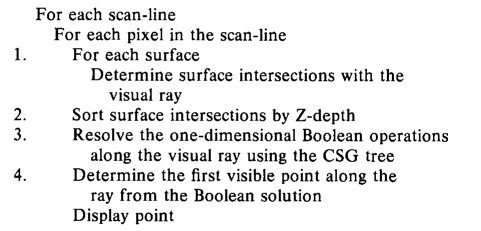
\includegraphics [scale=0.8] {1.png}
  \caption{Алгоритм бросания луча}
  \label{fig:roth_algo}
\end{figure}

В дополнение к простоте, метод имеет дополнительное преимущество для визуализации: после того как ближайшая точка определена, дальнейшие вычисления можно отбросить. Однако, перед тем как применить эти простые правила, необходимо пересечь луч с CSG примитивами и отсортировать точки пересечения. К тому же, все эти шаги должны быть выполнены для каждого пикселя изображения. \todo{[Roth]} описывает процедуру отсечения для уменьшения числа поверхностей, с которыми нужно пересечь луч для каждого пикселя. Однако, хотя такая оптимизация и дает эффект, тем не менее вычислительная сложность алгоритма не меняется. \todo{[Roth]} также приводит метод для определения и визуализации только силуэта и линий пересечения поверхностей, но этот метод не совместим с затененной визуализацией.

Широко используемый в то время (1980-е) для задачи определения видимости полигонов, построчный подход к визуализации (англ. scanline rendering), также был адаптирован для визуализации CSG моделей \todo{[atherton1983]}. Типичный scanline алгоритм, использующий Y-X-Z сортировку полигонов, представлен на рис. \ref{fig:atherton_algo}

\begin{figure} 
  \centering
  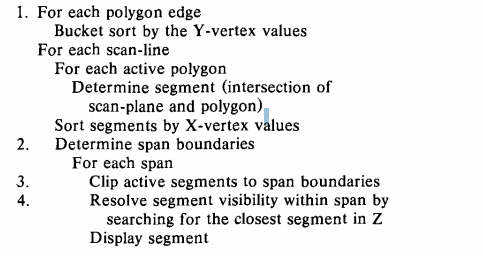
\includegraphics [scale=0.8] {scanline.png}
  \caption{Алгоритм scanline}
  \label{fig:atherton_algo}
\end{figure}

Сегментом в scanline алгоритмах называется часть полигона, образованная пересечением scanline плоскости и полигона.

Интервалом называется непрерывная часть scanline, для которой возможно определить видимый сегмент. 

Алгоритм, предложенный \todo{[atherton1983]} использует те же 4 шага, что и обычный алгоритм scanline, однако вместо определения видимости сегмента в интервале по его близости к виртуальной камере (наблюдателю), используется более сложная процедура, аналогичная процедуре поиска видимой поверхности с помощью трассировки луча, примененной к концам интервала. В случае, если для концов интервала видимыми становятся разные поверхности, интервал рекурсивно разбивается.

Как и во многих других исследованиях, посвещенных scanline алгоритмам, в работе \todo{[atherton1983]} была предпринята попытка использовать свойства когерентности геометрии для оптимизации вычислений. Когерентность интервалов можно считать первым улучшением по сравнению с трассировкой лучей. Если на границах интервала видима одна и та же поверхность, то и результаты расчета затенения можно интерполировать между концами интервала.

Все разнообразие алгоритмов визуализации CSG моделей можно разделить на три базовых подхода. Первый подход основан на предварительном расчете полной границы CSG объекта (переход к граничному представлению), которая затем тесселируется и визуализируется с использованием традиционных инструментов 3D графики (Direct3D, OpenGL). Поскольку расчет границы является  вычислительно трудоемкой операцией, алгоритмы данной группы зачастую применимы только для статических сцен и не позволяют выполнять интерактивное редактирование конструктивных моделей.

Второй подход основан на переходе к воксельному представлению, для этого достаточно иметь возможность классифицировать точку относительно CSG дерева. После этого геометрию можно визуализировать как 3Д текстуру, средствами объемного рендеринга (англ. volume rendering). К недостатком такого подхода можно отнести большой объем занимаемого пространства и ограниченную точность представления (шагом воксельной сетки). Однако такой подход достаточно прост и производительность визуализации не зависит от сложности CSG дерева. \todo{Hardware-based slicing algorithm for CSG [58, 44]}.

Третий подход построен на базе техник анализа изображения (англ. image-based), которые генерируют только изображение CSG модели с заданного ракурса, избегая трудоемких вычислений полной границы. Большинство таких методов разработано для графической аппаратуры и реализуется с помощью многопроходных и зависящих от ракурса техник, интенсивно использующих буферы глубины и трафарета. В рамках данного подхода широкое распространение получили алгоритм \todo{Goldfeather [1, 2]} и алгоритм последовательного вычитания выпуклых оболочек (англ. Sequenced Convex Subtraction, SCS) \todo{[3]}. Первый из них поддерживает любые CSG примитивы, в то время как второй применим только к сценам, состоящим из выпуклых примитивов. При этом ни один из указанных  алгоритмов не позволяет визуализировать конструктивные модели напрямую. Вместо этого, CSG выражение должно быть преобразовано в дизъюнктивную нормальную форму (дизъюнкция с минимальным числом элементарных конъюнкций), что может приводить к экспоненциальному росту размера булевой формулы, значительно ограничивая  масштабируемость и производительность алгоритмов. Позже был предложен алгоритм Improved Layered Goldfeather Algorithm (General purpose Z-buffer CSG rendering with consumer level hardware). Обзор техник, использующих буфер глубины, представлен в работе \todo{[93]}. Визуализация CSG моделей с использованием двустороннего теста глубины описанная в \todo{[42]} позволила улучшить разложение сцены по слоям, используя аппаратный тест глубины для расчета теней. В работе \todo{[52]} были предложены улучшения SCS алгоритма, закадровый (англ. off-screen) рендеринг, поддерживаемый теперь аппаратно, наряду с запросом видимости OpenGL (для вычисления количества слоев) позволили увеличить производительность метода. 3D-графическая библиотека \todo{OpenCSG [53]} реализует интерактивный рендеринг CSG с использованием таких алгоритмов как Goldfeather и SCS. 

Альтернативный подход был предложен в более поздней работе \cmd{[4]} и получил название Blister. Вместо нормальной формы, данный метод преобразует CSG формулу к списку BList \todo{[5]}, содержащему каждый примитив ровно один раз. Для визуализации заданной конструктивной модели Blister задействует многопроходную технику разложения сцены по слоям (англ. depth peeling), с помощью которой входная сцена разбивается на слои, все фрагменты которых имеют одинаковый индекс близости (занимают равные позиции в списке фрагментов, отсортированных по мере удаления от камеры). Точки каждого слоя классифицируются согласно заданному CSG выражению и комбинируются для синтеза окончательного изображения. Показано, что для модели с $k$ слоями глубины и $n$ примитивами алгоритм вычисляет изображение за время $O(kn)$. В худшем случае $k$ линейно зависит от $n$, поэтому трудоемкость следует оценить как $O(n^2)$.

Указанные выше алгоритмы обеспечивают интерактивное отображение конструктивных моделей малой или средней  сложности (от нескольких сотен до нескольких десятков тысяч примитивов). При этом их общей чертой является активное использование многопроходных схем, которые ставят скорость рендеринга в зависимость от пропускной способности памяти. На протяжении последних десяти лет пропускная способность памяти GPU растет значительно медленнее производительности вычислительных модулей,  что делает передачу данных узким местом во многих GPU алгоритмах.

Альтернативный подход к визуализации конструктивных сцен был предложен в работе [6], где была предпринята попытка распределения вычислений между центральным и графическим процессором. Для этого входное CSG дерево декомпозируется на простые составляющие (содержащие малое число примитивов), которые затем визуализируются на GPU методом трассировки лучей. Входной CSG объект разбивается до тех пор, пока отдельные его части не будут соответствовать одиночным CSG примитивам или булевой  комбинации двух примитивов. Очевидно, что некоторые фрагменты модели не могут быть разбиты согласно двум указанным случаям (области, содержащие вершины 3-ого и более высоких порядков). Такие фрагменты алгоритмом отбрасываются, что выражается в визуальных артефактах при попытке увеличить изображение на экране монитора. Хотя данный подход оказался эффективным для простых сцен (сотни примитивов), более сложные модели требуют разбиения на большое число простых частей, что ведет к значительному росту числа вызовов отрисовки (англ. draw call) и снижению производительности.

Трассировка лучей для поиска пересечения с целым CSG деревом также возможна и применяется довольно широко. Однако большинство подходов к визуализации CSG сцен требует расчета всех пересечений луча с составляющими объект примитивами. При этом луч разбивается на набор интервалов, соответствующих пересекаемым примитивам. Затем к ним применяются правила булевой алгебры для вычисления ближайшей точки, расположенной на границе конструктивного объекта. Поскольку луч следует пересечь со всеми примитивами сцены, данный алгоритм является крайне вычислительно затратным. Кроме того, он плохо приспособлен для графических процессоров, которые не имеют ресурсов для хранения такого числа интервалов для десятков тысяч лучей. Тем не менее, для относительно простых сцен “интервальная” трассировка лучей на GPU вполне возможна, что наглядно показано в работе \todo{[7]}. В любом случае, данный алгоритм плохо масштабируется с ростом сложности сцены и числа слоев (влияет на число интервалов).

Совершенно другой подход к визуализации CSG моделей  на базе трассировки лучей был представлен в работе \todo{[8]} и основан на поиске ближайших точек соударения лучей с  примитивами 3D сцены. Алгоритм использует концепцию конечного автомата для вычисления точки пересечения с границей CSG модели. При этом требуется, чтобы базовые примитивы были замкнутыми (допустимо обобщение для полупространств, заданных ориентированными поверхностями), имели согласованное поле нормалей и не содержали самопересечений. Элегантность решения и приемлемые ограничения позволяют довольно просто реализовать поддержку конструктивных моделей в любой программной системе, основанной на трассировке лучей. Хотя указанная работа не содержит упоминаний о практических испытаниях алгоритма, он представляется наилучшей основой для разработки специализированной версии для GPU.

\section{Ускоряющие структуры} \label{sect_acceleration_structures}

Для эффективной визуализации многие алгоритмы используют различные структуры данных, которые в контексте визуализации принято называть ускоряющими структурами (англ. acceleration structure). Ускоряющие структуры могут использоваться для пропуска пустого пространства в случае визуализации воксельных представлений. В подходах использующих растеризацию, ускоряющие структуры помогают отсекать невидимую геометрию. Особенно критичны ускоряющие структуры для трассировки лучей. Наиболее трудоемкой операцией в большинстве алгоритмов на базе трассировки лучей является поиск ближайшей точки пересечения луча с объектами сцены. Перед тестированием луча на пересечение с геометрией сцены определяется его пересечение с ускоряющей структурой (данная операция обычно называется «обходом»). В качестве результата ускоряющая структура возвращает ближайшую область пространства с подмножеством примитивов сцены. Процедура трассировки тестирует луч на пересечение с примитивами данного подмножества. Если точка соударения не обнаружена, то ускоряющая структура запрашивается повторно для получения нового подмножества примитивов. Этот процесс продолжается до тех пор, пока для луча не будет найдено соударение или не будет установлено, что данный луч не пересекает сцену.

Расчет точки пересечения луча с объектами сцены относится к задачам поиска, поэтому все ускоряющие структуры реализуют некоторый механизм пространственной сортировки объектов. С точки зрения базового подхода к сортировке все ускоряющие структуры можно разделить на два типа: разбиения пространства (англ. spatial subdivision) и иерархии объектов (англ. object hierarchy). Данные типы являются двойственными по своей природе. Разбиения пространства позволяют уникально представить каждую точку пространства, однако каждый примитив сцены может перекрываться любым числом ячеек. Иерархии объектов позволяют уникально представить каждый примитив, однако каждая точка сцены может перекрываться любым числом ячеек. Примерами разбиений пространства являются такие структуры, как регулярные \todo{[11]} или иерархические \todo{[12]} сетки, октодеревья \todo{[13]} и k-d деревья \todo{[14]}, которые отличаются степенью регулярности \todo{[15]}. Напротив, иерархии ограничивающих объемов \todo{[16]} и их варианты (такие как иерархии ограничивающих интервалов \todo{[17; 18]}) служат примерами иерархий объектов. Развитие методов трассировки лучей неразрывно связано с развитием ускоряющих структур, алгоритмов их построения и обхода. Подробному обзору ускоряющих структур и их относительной эффективности посвящена работа \todo{[19]}.
В большинстве случаев ускоряющие структуры строятся на этапе препроцессирования сцены, поэтому трудоемкость их построения не учитывается на этапе визуализации. Данный подход допустимо применять только для статических сцен (с неизменной геометрией), во время отображения которых возможны перемещения лишь виртуальной камеры и изменения источников света. Для обработки динамических сцен (с подвижной геометрией) необходимо выполнять повторное построение или частичное обновление ускоряющей структуры каждый раз при модификации объектов.